\chapter{Modelling Correlation Between Risks}

Copulae are an interesting mathematical tool to represent correlations between probability distributions. They can be used to represent complex dependencies in multivariate risk models, when more basic tools such as multivariate gaussian distributions are inappropriate. One commonly used application is sampling from correlated random variables.
The concept will be described in this chapter together with practical applications in computing default probabilities in multinamed contracts like CDOs and Basket Default Swaps.

\section{Copulae}

The definition of a \emph{copula} is: a multivariate distribution
\(C(U_1, U_2, \ldots, U_n)\) such that marginalizing gives
\(U_i \approx\)\textasciitilde{}Uniform(0,1). Despite this obscure and
daunting sentence the concept is quite simple so let's try to clarify it
a bit and at the end we will see what role copulas played in the 2008
financial crisis.

\subsection{Example Problem Case}\label{example-problem-case}

Imagine we measure two variables that are non-normally distributed and
correlated. For example, we look at various rivers and for every river
we look at the maximum level of that river over a certain time-period.
In addition, we also count how many months each river caused flooding.
For the probability distribution of the maximum level of the river we
know that maximums are \href{}{\emph{Grumbel}} distributed, while the
number of flooding can be modelled according to a \href{}{\emph{Beta}}
distribution.

Clearly it is pretty reasonable to assume that the maximum level and the
number of floodings is going to be correlated, however we don't know how
we could model that correlated probability distribution. Above we only
specified the distributions for individual variables, irrespective of
the other one (i.e.~the marginals), in reality we are dealing with a
joint distribution of both of these together.

And here is where copulas come to our rescue.

Copulas essentially allow to decompose a joint probability distribution
into their marginals (which by definition have no correlation) and a
function which couples (hence the name) them together and thus allows us
to specify the correlation separately. The copula is that coupling
function.

Before going into them, we must first learn how we can transform
arbitrary random variables to uniform and back.

\subsection{Distribution
Transformation}\label{distribution-transformation}

The technique we are going to use to transform every random variables to
uniform and viceversa is called \emph{probability integral transform}.
We won't go into the details but we will just show few examples of how
this can be done in \texttt{python} and we will use the
\texttt{scipy.stats} module to do the job.

So first, we sample uniformly distributed values between 0 and 1:

    \begin{tcolorbox}[breakable, size=fbox, boxrule=1pt, pad at break*=1mm,colback=cellbackground, colframe=cellborder]
\begin{Verbatim}[commandchars=\\\{\}]
\PY{k+kn}{from} \PY{n+nn}{scipy} \PY{k}{import} \PY{n}{stats}
\PY{k+kn}{from} \PY{n+nn}{matplotlib} \PY{k}{import} \PY{n}{pyplot} \PY{k}{as} \PY{n}{plt}

\PY{n}{x} \PY{o}{=} \PY{n}{stats}\PY{o}{.}\PY{n}{uniform}\PY{p}{(}\PY{l+m+mi}{0}\PY{p}{,} \PY{l+m+mi}{1}\PY{p}{)}\PY{o}{.}\PY{n}{rvs}\PY{p}{(}\PY{l+m+mi}{10000}\PY{p}{)}
\end{Verbatim}
\end{tcolorbox}

Next we want to transform these samples so that instead of uniform they
are normally distributed. The transform that does this is the inverse of
the cumulative density function (CDF) of the normal distribution which
we can get in \texttt{scipy.stats} with \texttt{ppf}.

\begin{tcolorbox}[breakable, size=fbox, boxrule=1pt, pad at break*=1mm,colback=cellbackground, colframe=cellborder]
\begin{Verbatim}[commandchars=\\\{\}]
\PY{n}{norm} \PY{o}{=} \PY{n}{stats}\PY{o}{.}\PY{n}{distributions}\PY{o}{.}\PY{n}{norm}\PY{p}{(}\PY{p}{)} \PY{c+c1}{\PYZsh{} get the normal distribution definition}
\PY{n}{x\PYZus{}trans} \PY{o}{=} \PY{n}{norm}\PY{o}{.}\PY{n}{ppf}\PY{p}{(}\PY{n}{x}\PY{p}{)}
\end{Verbatim}
\end{tcolorbox}

    \begin{figure}[h]
    \centering
    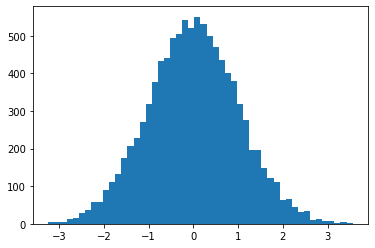
\includegraphics[width=0.6\textwidth]{copula_files/copula_3_0.png}
    \end{figure}
    
If we plot them together in a 2D plot we can get a sense of what is
going on using the inverse CDF transformation, see Fig.~\ref{fig:cdf_transform}.
The inverse CDF stretches the outer regions of the uniform to yield a
normal distribution.

    \begin{figure}[h]
\centering
    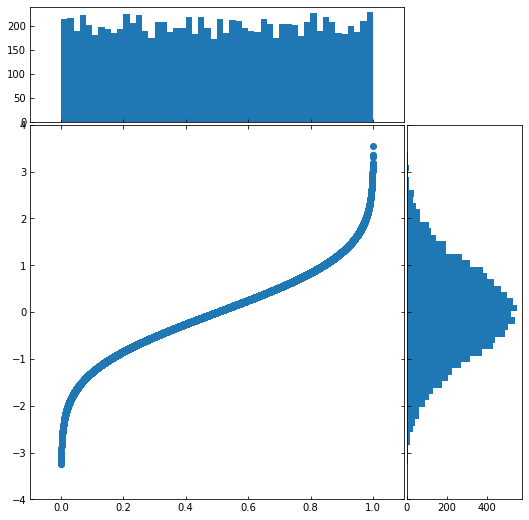
\includegraphics[width=0.6\textwidth]{copula_files/copula_5_0.png}
    \caption{2D plot showing the CDF transformation from uniform to Gaussian and viceversa.}
    \label{fig:cdf_transform}
    \end{figure}

    \begin{figure}[htbp]
\centering
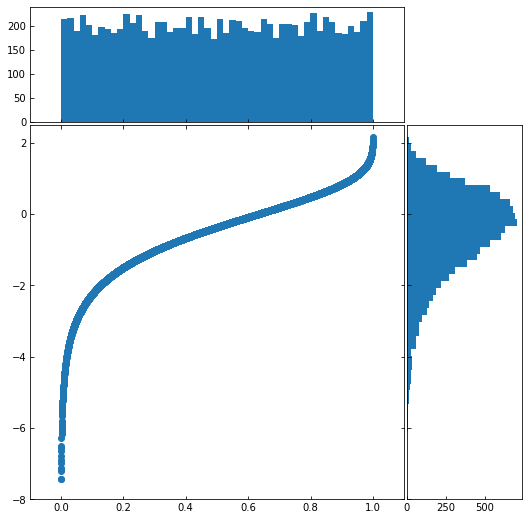
\includegraphics[width=0.6\textwidth]{copula_files/copula_7_0.png}
\caption{2D plot showing the CDF transformation from uniform to Gumbel and viceversa.}
\label{fig:2d_gumbel}
    \end{figure}

 The nice thing about this technique is that it can be
done for any arbitrary (univariate) probability distributions, like Beta
or Gumbel, see Fig.~\ref{fig:2d_gumbel}.

\begin{tcolorbox}[breakable, size=fbox, boxrule=1pt, pad at break*=1mm,colback=cellbackground, colframe=cellborder]
\begin{Verbatim}[commandchars=\\\{\}]
\PY{n}{gumbel} \PY{o}{=} \PY{n}{stats}\PY{o}{.}\PY{n}{distributions}\PY{o}{.}\PY{n}{gumbel\PYZus{}l}\PY{p}{(}\PY{p}{)}
\PY{n}{x\PYZus{}trans} \PY{o}{=} \PY{n}{gumbel}\PY{o}{.}\PY{n}{ppf}\PY{p}{(}\PY{n}{x}\PY{p}{)}
\end{Verbatim}
\end{tcolorbox}       

    Clearly to do the opposite transformation from an arbitrary distribution
to the uniform(0, 1) we can just apply the inverse of the inverse CDF,
the CDF itself\ldots

\subsection{Adding Correlation with Gaussian
Copulas}\label{adding-correlation-with-gaussian-copulas}

How does this help us with our problem of creating a custom joint
probability distribution ? We are actually almost done already, we know
how to convert anything uniformly distributed to an arbitrary
probability distribution. So that means we need to generate uniformly
distributed data with the correlation we want and then transform the
marginals into the desired distributions. How do we do that ? We
simulate from a multivariate Gaussian with the specific correlation
structure, transform so that the marginals are uniform, and then
transform the uniform marginals to whatever we like.

Generate random samples from multivariate normal with correlation 0.5 (Fig.~\ref{fig:gausswithcorr}):
       \begin{figure}[htbp]
    \centering
    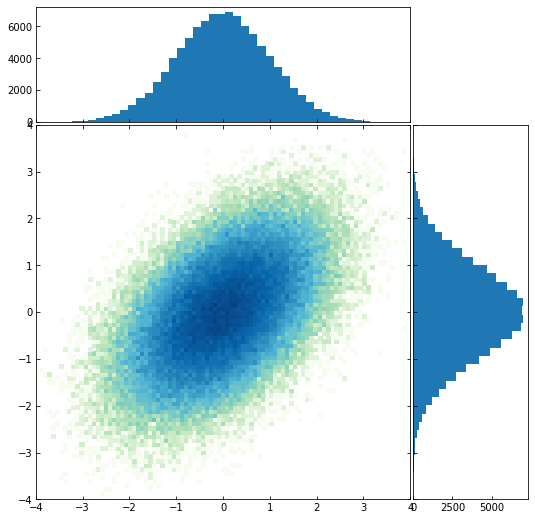
\includegraphics[width=0.6\textwidth]{copula_files/copula_9_0.png}
    \caption{2D plot showing the joint distribution of two Gaussian with a correlation factor of 0.5.}
    \label{fig:gausswithcorr}
    \end{figure}
 
\begin{tcolorbox}[breakable, size=fbox, boxrule=1pt, pad at break*=1mm,colback=cellbackground, colframe=cellborder]
\begin{Verbatim}[commandchars=\\\{\}]
\PY{c+c1}{\PYZsh{} this import is for plotting}
\PY{k+kn}{from} \PY{n+nn}{matplotlib} \PY{k}{import} \PY{n}{colors}

\PY{n}{mvnorm} \PY{o}{=} \PY{n}{stats}\PY{o}{.}\PY{n}{multivariate\PYZus{}normal}\PY{p}{(}\PY{n}{mean}\PY{o}{=}\PY{p}{[}\PY{l+m+mi}{0}\PY{p}{,} \PY{l+m+mi}{0}\PY{p}{]} \PY{p}{,} \PY{n}{cov}\PY{o}{=}\PY{p}{[}\PY{p}{[}\PY{l+m+mi}{1}\PY{p}{,} \PY{l+m+mf}{0.5}\PY{p}{]}\PY{p}{,}
                                                      \PY{p}{[}\PY{l+m+mf}{0.5}\PY{p}{,} \PY{l+m+mi}{1}\PY{p}{]}\PY{p}{]}\PY{p}{)}
\PY{n}{x} \PY{o}{=} \PY{n}{mvnorm}\PY{o}{.}\PY{n}{rvs}\PY{p}{(}\PY{l+m+mi}{100000}\PY{p}{)}
\end{Verbatim}
\end{tcolorbox}

    Now use what we have just seen to \emph{uniformify} the marginals:

    \begin{tcolorbox}[breakable, size=fbox, boxrule=1pt, pad at break*=1mm,colback=cellbackground, colframe=cellborder]
\begin{Verbatim}[commandchars=\\\{\}]
\PY{n}{norm} \PY{o}{=} \PY{n}{stats}\PY{o}{.}\PY{n}{norm}\PY{p}{(}\PY{p}{)}
\PY{n}{x\PYZus{}unif} \PY{o}{=} \PY{n}{norm}\PY{o}{.}\PY{n}{cdf}\PY{p}{(}\PY{n}{x}\PY{p}{)}
\end{Verbatim}
\end{tcolorbox}

    \begin{figure}
    \centering
    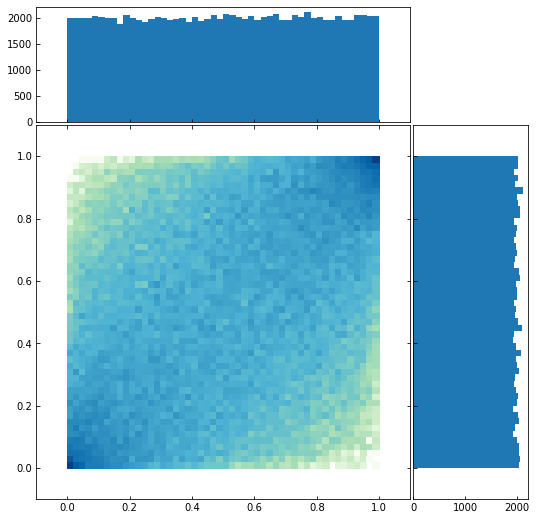
\includegraphics[width=0.4\textwidth]{copula_files/copula_11_0.png}
    \hspace{5mm}
    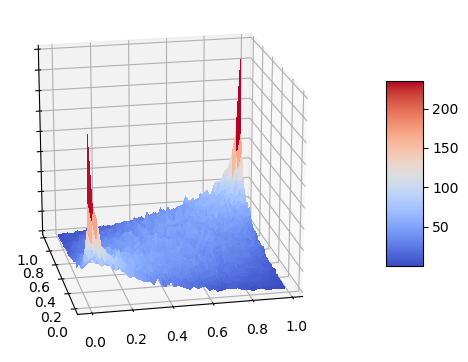
\includegraphics[width=0.5\textwidth]{copula_3d.png}
    \caption{Graphical representations of the copula, 2D on the left, 3D on the right.}
    \label{fig:copula}
    \end{figure}
    This scatter plot of Fig.~\ref{fig:copula} is usually how copulas are visualized. 
    
 Finally we can just transform the marginals again from uniform to what we want
(e.g.~Gumbel and Beta), see Fig.~\ref{fig:beta_gumbel_corr}:

    \begin{tcolorbox}[breakable, size=fbox, boxrule=1pt, pad at break*=1mm,colback=cellbackground, colframe=cellborder]
\begin{Verbatim}[commandchars=\\\{\}]
\PY{n}{m1} \PY{o}{=} \PY{n}{stats}\PY{o}{.}\PY{n}{gumbel\PYZus{}l}\PY{p}{(}\PY{p}{)}
\PY{n}{m2} \PY{o}{=} \PY{n}{stats}\PY{o}{.}\PY{n}{beta}\PY{p}{(}\PY{n}{a}\PY{o}{=}\PY{l+m+mi}{10}\PY{p}{,} \PY{n}{b}\PY{o}{=}\PY{l+m+mi}{3}\PY{p}{)}

\PY{n}{x1\PYZus{}trans} \PY{o}{=} \PY{n}{m1}\PY{o}{.}\PY{n}{ppf}\PY{p}{(}\PY{n}{x\PYZus{}unif}\PY{p}{[}\PY{p}{:}\PY{p}{,} \PY{l+m+mi}{0}\PY{p}{]}\PY{p}{)}
\PY{n}{x2\PYZus{}trans} \PY{o}{=} \PY{n}{m2}\PY{o}{.}\PY{n}{ppf}\PY{p}{(}\PY{n}{x\PYZus{}unif}\PY{p}{[}\PY{p}{:}\PY{p}{,} \PY{l+m+mi}{1}\PY{p}{]}\PY{p}{)}
\end{Verbatim}
\end{tcolorbox}

    \begin{figure}[htbp]
    \centering
    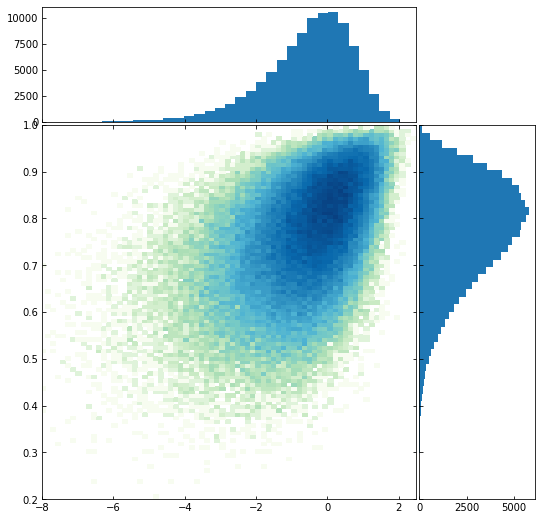
\includegraphics[width=0.6\textwidth]{copula_files/copula_13_0.png}
    \caption{Marginalized Gumbel and Beta distribution with Gaussian copula correlation.}
    \label{fig:beta_gumbel_corr}
    \end{figure}
    
    It is now interesting to compare with the joint distribution without
correlations, see Fig.~\ref{fig:beta_gumbel_nocorr}:

    \begin{tcolorbox}[breakable, size=fbox, boxrule=1pt, pad at break*=1mm,colback=cellbackground, colframe=cellborder]
\begin{Verbatim}[commandchars=\\\{\}]
\PY{n}{x1} \PY{o}{=} \PY{n}{m1}\PY{o}{.}\PY{n}{rvs}\PY{p}{(}\PY{l+m+mi}{10000}\PY{p}{)}
\PY{n}{x2} \PY{o}{=} \PY{n}{m2}\PY{o}{.}\PY{n}{rvs}\PY{p}{(}\PY{l+m+mi}{10000}\PY{p}{)}
\end{Verbatim}
\end{tcolorbox}

    \begin{figure}[htbp]
    \centering
    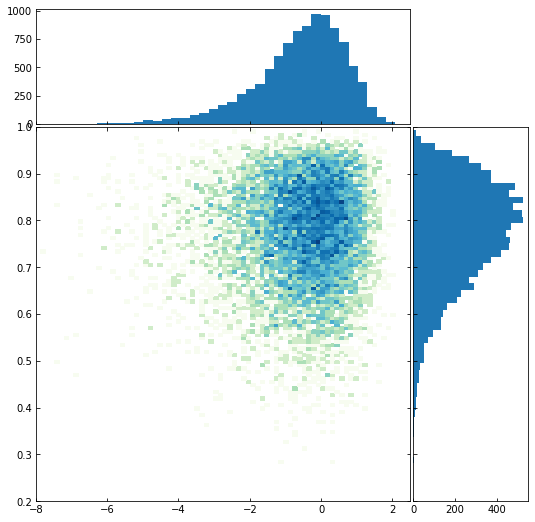
\includegraphics[width=0.6\textwidth]{copula_files/copula_15_0.png}
    \caption{Marginalized Gumbel and Beta distribution without Gaussian copula correlation.}
    \label{fig:beta_gumbel_nocorr}
    \end{figure}
    
    Using the uniform distribution as a common base for our transformations
we can easily introduce correlations and flexibly construct complex
probability distributions. Clearly this is directly extendeable to
higher dimensional distributions as well.

\section{Application to Finance}\label{application-to-finance}

In credit derivative valuation and credit risk management, one of the
fundamentally important issues is the estimation of default
probabilities and their correlations. For this, generally speaking,
there are two ways: using historical default data or using mathematical
models.

Historical default data has played an important role in the estimation
of default probabilities. However, because default events are rare,
there is very limited default data available. Moreover, historical data
reflects the historical default pattern only and it may not be a proper
indicator of the future. This makes the estimation of default
probabilities from historical data difficult and inexact. To use this
same data to estimate default correlations is even more difficult and
more inexact.

The market trend now is towards more and more to the use of mathematical
models that don't rely on historical default data. In the previous
chapter we have seen how it is possible to derive default probabilities
from market data. Before going into the details of the application of
the copula to default probabilities let's introduce two more kind of
contracts.

\subsection{Basket Default Swaps}\label{basket-default-swaps}

A basket default swap is a credit derivative on a portfolio of reference
entities. The simplest basket default swaps are first-to-default swaps,
second-to-default swaps, and nth-to-default swaps. With respect to a
basket of reference entities, a first-to-default swap provides insurance
for only the first default, a second-to-default swap provides insurance
for only the second default, an nth-to-default swap provides insurance
for only the nth default. For example, in an nth-to-default swap, the
protection seller does not make a payment to the protection buyer for
the first n-defaulted reference entities, and makes a payment for the
nth defaulted reference entity. Once there is a payment upon the
default of the nth defaulted reference entity, the swap terminates.

\subsubsection{Collateralized Debt Obligation}\label{collateralized-debt-obligation}

A collateralized debt obligation (CDO) is a security backed by a
diversified pool of one or more kinds of debt obligations such as bonds,
loans, credit default swaps or structured products (mortgage-backed
securities, asset-backed securities, and even other CDOs). A CDO can be
initiated by one or more of the following: banks, nonbank financial
institutions, and asset management companies, is referred to as the
sponsor. The sponsor of a CDO creates a company so-called the special
purpose vehicle (SPV). The SPV works as an independent entity. In this
way, CDO investors are isolated from the credit risk of the sponsor.
Moreover, the SPV is responsible for the administration. The SPV obtains
the credit risk exposure by purchasing debt obligations (bonds or
residential and commercial loans) or selling CDSs; it transfers the
credit risk by issuing debt obligations (tranches/credit-linked notes).
The investors in the tranches of a CDO have the ultimate credit risk
exposure to the underlying reference entities. The SPV issues four kinds
of tranches. Each tranche has an attachment percentage and a detachment
percentage. When the cumulative percentage loss of the portfolio reaches
the attachment percentage, investors in the tranche start to lose their
principal, and when the cumulative percentage loss of principal reaches
the detachment percentage, the investors in the tranche lose all their
principal and no further loss can occur to them.

In the literature, tranches of a CDO are classified as
subordinate/equity tranche, mezzanine tranches, and senior tranches
according to their subordinate levels. Because the equity tranche is
extremely risky, the sponsor of a CDO holds the equity tranche and the
SPV sells other tranches to investors.

\subsection{Calculating $n$th-to-default probability}\label{calculating-first-to-default-nth-to-default-and-all-to-default-probabilities}

\subsubsection{Independent Defaults}\label{independent-defaults}

If the default times of the names of a basket are independent,
first-to-default, nth-to-default, all-to-default probabilities can be
calculated through multiplication and integration of the default
probability curves of the basket components.

As an example, we consider the second-to-default probability of a 4-name
basket. Let \(\tau_i\) be the default time of name \(i\) and \(F_i(t)\)
its distribution. Then the probability that name 1 defaults second in
the basket before time \(t\) and before the counter-party defaults:

\begin{equation*}
\begin{split}
&\mathbb{P}((\tau_2\lt\tau_1)\cap (\tau_1\lt t)\cap (\tau_1\lt\tau_3)\cap (\tau_1\lt\tau_4)) +\\
&\mathbb{P}((\tau_3\lt\tau_1)\cap (\tau_1\lt t)\cap (\tau_1\lt\tau_2)\cap (\tau_1\lt\tau_4)) =\\
&\int_0^t{F_2 (s)\cdot (1-F_3 (s)) \cdot (1-F_4 (s))~dF_1(s)} +  \int_0^t{F_3 (s)\cdot (1-F_2 (s)) \cdot (1-F_4 (s))~dF_1(s)}
\end{split}
\end{equation*}

The formula for nth-to-default probability before the counter-party
defaults in a general basket can be derived similarly. However,
complexity increases as the number of names increases. The above method
can also apply to derive the formula of all-to-default probability
before the counter-party defaults. This is clearly much simpler than the
nth-to-default case.

Suppose the default probabilities of three companies, A, B and C are
given as in the following table:

\begin{center}
\begin{tabular}{|c|c|c|c|}
time in years & A & B & C \\
\hline
0 & 0 & 0 & 0 \\
1 & 0.022032 & 0.0317 & 0.035 \\
2 & 0.046242 & 0.0655 & 0.075 \\
3 & 0.07266 & 0.1022 & 0.121 \\
4 & 0.101233 & 0.142 & 0.153 \\
5 & 0.131885 & 0.1752 & 0.205 \\
\end{tabular}
\end{center}

and suppose that the default events of the three companies are
independent. Using linear interpolation for default probability curves,
let's get the table of first-to-default probabilities for the three
companies.

The default probabilities are linear in each time interval so the
integral above can be solved by substitution:

\[ \int_{x_0}^{x_1}{(1-F_B(x))(1-F_C(x))dF_A(x)}\]

Setting \(t=m_A x + q_A\) it becomes with \(m_A, q_A\) are the
parameters of the line joining the default probabilities of company A:

\[ \int_{m_A x_0 + q_A}^{m_A x_1 + q_A}{(1-F_B(x(t)))(1-F_C(x(t)))dt}~~~~~~\Big(\textrm{with}~x(t) = \cfrac{t -q_A}{m_A}\Big) \]
and similarly for company B and C.

To convert it into python we can use \texttt{scipy.integrate.quad} to
perform the integral and \texttt{numpy.interp} to determine the
intermediate default probabilities.

    \begin{tcolorbox}[breakable, size=fbox, boxrule=1pt, pad at break*=1mm,colback=cellbackground, colframe=cellborder]
\begin{Verbatim}[commandchars=\\\{\}]
\PY{k+kn}{from} \PY{n+nn}{scipy}\PY{n+nn}{.}\PY{n+nn}{integrate} \PY{k}{import} \PY{n}{quad}
\PY{k+kn}{from} \PY{n+nn}{numpy} \PY{k}{import} \PY{n}{interp}

\PY{n}{default\PYZus{}rates} \PY{o}{=} \PY{p}{\PYZob{}}\PY{l+s+s2}{\PYZdq{}}\PY{l+s+s2}{A}\PY{l+s+s2}{\PYZdq{}}\PY{p}{:}\PY{p}{(}\PY{l+m+mi}{0}\PY{p}{,} \PY{l+m+mf}{0.022032}\PY{p}{,} \PY{l+m+mf}{0.046242}\PY{p}{,} \PY{l+m+mf}{0.07266}\PY{p}{,} \PY{l+m+mf}{0.101233}\PY{p}{,} \PY{l+m+mf}{0.131885}\PY{p}{)}\PY{p}{,}
                 \PY{l+s+s2}{\PYZdq{}}\PY{l+s+s2}{B}\PY{l+s+s2}{\PYZdq{}}\PY{p}{:}\PY{p}{(}\PY{l+m+mi}{0}\PY{p}{,} \PY{l+m+mf}{0.0317}\PY{p}{,} \PY{l+m+mf}{0.0655}\PY{p}{,} \PY{l+m+mf}{0.1022}\PY{p}{,} \PY{l+m+mf}{0.142}\PY{p}{,} \PY{l+m+mf}{0.1752}\PY{p}{)}\PY{p}{,}
                 \PY{l+s+s2}{\PYZdq{}}\PY{l+s+s2}{C}\PY{l+s+s2}{\PYZdq{}}\PY{p}{:}\PY{p}{(}\PY{l+m+mi}{0}\PY{p}{,} \PY{l+m+mf}{0.035}\PY{p}{,} \PY{l+m+mf}{0.075}\PY{p}{,} \PY{l+m+mf}{0.121}\PY{p}{,} \PY{l+m+mf}{0.153}\PY{p}{,} \PY{l+m+mf}{0.205}\PY{p}{)}\PY{p}{\PYZcb{}}

\PY{k}{def} \PY{n+nf}{func}\PY{p}{(}\PY{n}{x}\PY{p}{,} \PY{n}{default}\PY{p}{,} \PY{n}{companies}\PY{p}{,} \PY{n}{t}\PY{p}{)}\PY{p}{:}
    \PY{n}{m} \PY{o}{=} \PY{n}{default}\PY{p}{[}\PY{n}{companies}\PY{p}{[}\PY{l+m+mi}{0}\PY{p}{]}\PY{p}{]}\PY{p}{[}\PY{n}{t}\PY{p}{]} \PY{o}{\PYZhy{}} \PY{n}{default}\PY{p}{[}\PY{n}{companies}\PY{p}{[}\PY{l+m+mi}{0}\PY{p}{]}\PY{p}{]}\PY{p}{[}\PY{n}{t}\PY{o}{\PYZhy{}}\PY{l+m+mi}{1}\PY{p}{]}
    \PY{n}{q} \PY{o}{=} \PY{n}{default}\PY{p}{[}\PY{n}{companies}\PY{p}{[}\PY{l+m+mi}{0}\PY{p}{]}\PY{p}{]}\PY{p}{[}\PY{n}{t}\PY{o}{\PYZhy{}}\PY{l+m+mi}{1}\PY{p}{]} \PY{o}{\PYZhy{}} \PY{n}{m} \PY{o}{*} \PY{p}{(}\PY{n}{t}\PY{o}{\PYZhy{}}\PY{l+m+mi}{1}\PY{p}{)}
    \PY{n}{t} \PY{o}{=} \PY{p}{(}\PY{n}{x}\PY{o}{\PYZhy{}}\PY{n}{q}\PY{p}{)}\PY{o}{/}\PY{n}{m}
    \PY{n}{F2} \PY{o}{=} \PY{l+m+mi}{1} \PY{o}{\PYZhy{}} \PY{n}{interp}\PY{p}{(}\PY{n}{t}\PY{p}{,} \PY{n+nb}{range}\PY{p}{(}\PY{n+nb}{len}\PY{p}{(}\PY{n}{default}\PY{p}{[}\PY{n}{companies}\PY{p}{[}\PY{l+m+mi}{1}\PY{p}{]}\PY{p}{]}\PY{p}{)}\PY{p}{)}\PY{p}{,} \PY{n}{default}\PY{p}{[}\PY{n}{companies}\PY{p}{[}\PY{l+m+mi}{1}\PY{p}{]}\PY{p}{]}\PY{p}{)}
    \PY{n}{F3} \PY{o}{=} \PY{l+m+mi}{1} \PY{o}{\PYZhy{}} \PY{n}{interp}\PY{p}{(}\PY{n}{t}\PY{p}{,} \PY{n+nb}{range}\PY{p}{(}\PY{n+nb}{len}\PY{p}{(}\PY{n}{default}\PY{p}{[}\PY{n}{companies}\PY{p}{[}\PY{l+m+mi}{2}\PY{p}{]}\PY{p}{]}\PY{p}{)}\PY{p}{)}\PY{p}{,} \PY{n}{default}\PY{p}{[}\PY{n}{companies}\PY{p}{[}\PY{l+m+mi}{2}\PY{p}{]}\PY{p}{]}\PY{p}{)}
    \PY{k}{return} \PY{n}{F2}\PY{o}{*}\PY{n}{F3}

\PY{k}{def} \PY{n+nf}{integral}\PY{p}{(}\PY{n}{default}\PY{p}{,} \PY{n}{companies}\PY{p}{,} \PY{n}{t}\PY{p}{)}\PY{p}{:}
    \PY{k}{return} \PY{n}{quad}\PY{p}{(}\PY{n}{func}\PY{p}{,} \PY{l+m+mi}{0}\PY{p}{,} \PY{n}{default}\PY{p}{[}\PY{n}{companies}\PY{p}{[}\PY{l+m+mi}{0}\PY{p}{]}\PY{p}{]}\PY{p}{[}\PY{n}{t}\PY{p}{]}\PY{p}{,} 
                                          \PY{n}{args}\PY{o}{=}\PY{p}{(}\PY{n}{default}\PY{p}{,} \PY{n}{companies}\PY{p}{,} \PY{n}{t}\PY{p}{)}\PY{p}{)}\PY{p}{[}\PY{l+m+mi}{0}\PY{p}{]}
                 
\PY{k}{for} \PY{n}{companies} \PY{o+ow}{in} \PY{p}{[}\PY{p}{(}\PY{l+s+s2}{\PYZdq{}}\PY{l+s+s2}{A}\PY{l+s+s2}{\PYZdq{}}\PY{p}{,} \PY{l+s+s2}{\PYZdq{}}\PY{l+s+s2}{B}\PY{l+s+s2}{\PYZdq{}}\PY{p}{,} \PY{l+s+s2}{\PYZdq{}}\PY{l+s+s2}{C}\PY{l+s+s2}{\PYZdq{}}\PY{p}{)}\PY{p}{,} \PY{p}{(}\PY{l+s+s2}{\PYZdq{}}\PY{l+s+s2}{B}\PY{l+s+s2}{\PYZdq{}}\PY{p}{,} \PY{l+s+s2}{\PYZdq{}}\PY{l+s+s2}{A}\PY{l+s+s2}{\PYZdq{}}\PY{p}{,} \PY{l+s+s2}{\PYZdq{}}\PY{l+s+s2}{C}\PY{l+s+s2}{\PYZdq{}}\PY{p}{)}\PY{p}{,} \PY{p}{(}\PY{l+s+s2}{\PYZdq{}}\PY{l+s+s2}{C}\PY{l+s+s2}{\PYZdq{}}\PY{p}{,} \PY{l+s+s2}{\PYZdq{}}\PY{l+s+s2}{A}\PY{l+s+s2}{\PYZdq{}}\PY{p}{,} \PY{l+s+s2}{\PYZdq{}}\PY{l+s+s2}{B}\PY{l+s+s2}{\PYZdq{}}\PY{p}{)}\PY{p}{]}\PY{p}{:}
    \PY{n}{prob} \PY{o}{=} \PY{l+m+mi}{0}
    \PY{k}{for} \PY{n}{t} \PY{o+ow}{in} \PY{n+nb}{range}\PY{p}{(}\PY{l+m+mi}{1}\PY{p}{,} \PY{l+m+mi}{6}\PY{p}{)}\PY{p}{:}
        \PY{n}{prob} \PY{o}{=} \PY{n}{integral}\PY{p}{(}\PY{n}{default\PYZus{}rates}\PY{p}{,} \PY{n}{companies}\PY{p}{,} \PY{n}{t}\PY{p}{)}
        \PY{n+nb}{print} \PY{p}{(}\PY{l+s+s2}{\PYZdq{}}\PY{l+s+s2}{P(1st def) at time (}\PY{l+s+si}{\PYZob{}\PYZcb{}}\PY{l+s+s2}{) for company }\PY{l+s+si}{\PYZob{}\PYZcb{}}\PY{l+s+s2}{: }\PY{l+s+si}{\PYZob{}:.5f\PYZcb{}}\PY{l+s+s2}{\PYZdq{}}\PY{o}{.}\PY{n}{format}\PY{p}{(}\PY{n}{t}\PY{p}{,} 
              					  \PY{n}{companies}\PY{p}{[}\PY{l+m+mi}{0}\PY{p}{]}\PY{p}{,} \PY{n}{prob}\PY{p}{)}\PY{p}{)}
\end{Verbatim}
\end{tcolorbox}

    \begin{Verbatim}[commandchars=\\\{\}]
First to default prob at time (1) for company A: 0.02131
First to default prob at time (2) for company A: 0.04301
First to default prob at time (3) for company A: 0.06460
First to default prob at time (4) for company A: 0.08573
First to default prob at time (5) for company A: 0.10606
First to default prob at time (1) for company B: 0.03080
First to default prob at time (2) for company B: 0.06160
First to default prob at time (3) for company B: 0.09245
First to default prob at time (4) for company B: 0.12315
First to default prob at time (5) for company B: 0.15018
First to default prob at time (1) for company C: 0.03407
First to default prob at time (2) for company C: 0.07071
First to default prob at time (3) for company C: 0.10986
First to default prob at time (4) for company C: 0.13879
First to default prob at time (5) for company C: 0.17011
    \end{Verbatim}

\subsection{Correlated Defaults}\label{correlated-defaults}
The cost of protection in $k$th-to-default CDS or a tranche of CDOs is critically dependent
on a default correlation. Suppose that a basket of 100 reference entities is used to define a 5-year
$k$th-to-default CDS and that each reference entity has a probability of 2\% of defaulting during the 
5 years. When the default correlation between the reference entities is zero the binomial distribution 
shows that the probability of one or more defaults during 5 years is 86.74\% and a probability of 
10 or more defaults is 0.0034\%.

\begin{tcolorbox}[breakable, size=fbox, boxrule=1pt, pad at break*=1mm,colback=cellbackground, colframe=cellborder]
\begin{Verbatim}[commandchars=\\\{\}]
\PY{k+kn}{from} \PY{n+nn}{scipy}\PY{n+nn}{.}\PY{n+nn}{stats} \PY{k}{import} \PY{n}{binom}

\PY{n}{b} \PY{o}{=} \PY{n}{binom}\PY{p}{(}\PY{l+m+mi}{100}\PY{p}{,} \PY{l+m+mf}{0.02}\PY{p}{)}
\PY{n+nb}{print}\PY{p}{(}\PY{l+s+s2}{\PYZdq{}}\PY{l+s+s2}{P(\PYZgt{}=1) : }\PY{l+s+si}{\PYZob{}\PYZcb{}}\PY{l+s+s2}{\PYZdq{}}\PY{o}{.}\PY{n}{format}\PY{p}{(}\PY{l+m+mi}{1} \PY{o}{\PYZhy{}} \PY{n}{b}\PY{o}{.}\PY{n}{cdf}\PY{p}{(}\PY{l+m+mi}{0}\PY{p}{)}\PY{p}{)}\PY{p}{)}
\PY{n+nb}{print}\PY{p}{(}\PY{l+s+s2}{\PYZdq{}}\PY{l+s+s2}{P(\PYZgt{}=10): }\PY{l+s+si}{\PYZob{}\PYZcb{}}\PY{l+s+s2}{\PYZdq{}}\PY{o}{.}\PY{n}{format}\PY{p}{(}\PY{l+m+mi}{1} \PY{o}{\PYZhy{}} \PY{n}{b}\PY{o}{.}\PY{n}{cdf}\PY{p}{(}\PY{l+m+mi}{9}\PY{p}{)}\PY{p}{)}\PY{p}{)}

P(>=1) : 0.8673804441052471
P(>=10): 3.441680604299169e-05
\end{Verbatim}
\end{tcolorbox}

A first-to-default is therefore quite valuable whereas a tenth-to-default CDS is worth almost nothing.

As the default correlation increases the probability of one or more defaults declines and the probability 
of 10 or more defaults increases. In the limit where the default correlation is perfect the probability of one 
or more defaults equals the probability of ten or more defaults and it is 2\%. This is because in this extreme
situation the reference entities are essentially the same : either they all default (with 2\% probability) or none of them default (with 98\% probability).

To determine \(k\)th-to-default in case of correlated probabilities the
copula technique connected to Monte Carlo simulation can be used. The
most commonly used copula is the normal copula. which is simply a
function of a multi-dimensional normal distribution:

\[C(x_1,\ldots,x_m) = \Phi_m(\Phi^{-1}_1(x_1),\ldots,\Phi^{-1}_1(x_m), \rho) \]
where

\begin{itemize}
\tightlist
\item
  \(C\) is an m-dimensional copula;
\item
  \(\Phi_m\) is the distribution function of an \(k\)-dimensional normal
  random vector with a mean vector of \((0,\ldots,0)\) and a standard
  deviation vector of \((1,\dots,1)\);
\item
  \(\rho\) is the correlation matrix;
\item
  \(\Phi^{-1}\) is the inverse of the one-dimensional standard normal
  distribution.
\end{itemize}

Let \(\tau_i\) and \(F_i\) be the default time and its distribution of
name \(i\). To consider the default correlation of the basket (i.e.~the
correlations of the default times), we assume that the joint
distribution of the default times is:

\[\mathbb{P}(\tau_1 <t_1,\ldots, \tau_m <t_m) = C(F_1(t_1),\ldots, F_m(t_m))\]

where the correlation matrix of the m-dimensional distribution
underlying the normal copula is the asset correlation matrix of the
basket.

The right hand side of the above formula has a closed form and looks
quite appealing. Unfortunately, its calculation involves integration
over a multi-dimensional space. Numerical methods for the calculation of
such an integration are not sufficiently fast. Hence Monte Carlo
simulation has to be used.

Here are the steps to calculate the probability that name \(i\) is the
\(k\)th-to-default before time \(t\).

\begin{itemize}
\tightlist
\item
  Generate an m-dimensional random vector \(Z_1,\ldots,Z_m\) from the
  distribution \(\Phi_m\);
\item
  calculate \(\tau_i=F^{-1}(\Phi_1(Z_i))\) for each \(i\);
\item
  sort \(\tau_i\) in increasing order;
\item
  check if \(\tau_i\) is \(k\)th and \(\tau_k \le t\).
\item
  count the number of times that the above is true and then calculate
  the probability required.
\end{itemize}

\section{Gaussian Copula Model for Time to Default}
The critical input into pricing a synthetic CDO tranches or Basket CDS is an estimate of the default dependence (default correlation) between the underlying assets.
One popular method for estimating the dependence structure is using copula functions, a method first applied in actuarial science. While there are several types of copula function models, the first introduced was the one-factor Gaussian copula
model.

Suppose that a CDO includes $n$ assets $i = 1, 2,\ldots, n$ and the default times $\tau_i$ of
the $i$th asset follows a Poisson process with a parameter $\lambda_i$. The $\lambda_i$ is the default
intensity of the $i$th asset. Then the probability of a default occurring before the
time $t$ is

\[\mathbb{P}(\tau_i \lt t) = 1 - \mathrm{exp}(-\lambda_i t)\]

In a one-factor copula model, it is assumed that the default time $\tau_i$ for the $i$th
company is related to a random variable $X_i$ with a zero mean and a unit variance.
For any given time $t$, there is a corresponding value $x$ such that

\[\mathbb{P}(X_i < x) = \mathbb{P}(\tau_i < t),\qquad i = 1, 2,\ldots, n\]

Moreover, the one-factor copula model assumes that each random variable $X_i$ is the
sum of two components

\[X_i = a_i M + \sqrt{1-a_i^2 Z_i},\qquad i = 1, 2,\ldots, n\]

where $Z_i$ is the idiosyncratic component of company $i$, and $M$ is the common component of the market. It is assumed that the $M$ and $Z_i$ are mutually independent random variables. For simplicity, it is also assumed that the random variables $M$
and $Z_i$ are identical. The factor $a_i$ satisfies $-1 \le a_i \le 1$. The default correlation
between $X_i$ and $X_j$ is $a_i a_j,(i \ne j)$.

Let $F$ denote the cumulative distribution of the $Z_i$ and $G$ denote the cumulative distribution of the $X_i$. Then given the market condition $M = m$, we have

\[\mathbb{P}(Z_i < x|M = m) = F\left(\cfrac{x-a_i m}{\sqrt{1-a_i^2}}\right)\]
and the conditional default probability is

\[\mathbb{P}(\tau_i < t|M = m) = D_{t_i |m} = F\left\{\cfrac{G^{-1}[\mathbb{P}(\tau_i < t)] - a_i m}{\sqrt{1-a_i^2}}\right\}\]

For simplicity, the following two assumptions are made:
\begin{itemize}
\item all the companies have the same default intensity, i.e, $\lambda_i = \lambda$;
\item the pairwise default correlations are the same, i.e $a_i = a$.
\end{itemize}
The second assumption means that the contribution of the market component is
the same for all the companies and the correlation between any two companies is
constant, $\rho = a^2$.

Under these assumptions, given the market situation $M = m$, all the companies
have the same cumulative default probability $D_{t|m}$. Moreover, for a
given value of the market component $M$, the defaults are mutually independent for
all the underlying companies. Letting $N_{t|m}$ be the total defaults that have occurred
by time $t$ conditional on the market condition $M = m$, then $N_{t|m}$ follows a binomial
distribution, and

\[\mathbb{P}(N_{t|m} = j) = \cfrac{n!}{j!(n-j)!}D^j_{t|m}(1-D_{t|m})^{n-j},\qquad  j=0, 1, 2,\ldots,n\]
The probability that there will be exactly $j$ defaults by time $t$ is

\[\mathbb{P}(N_{t} = j) = \int_{-\infty}^{\infty}{\mathbb{P}(N_{t|m} = j)f_M(m)dm}\]
where $f_M(m)$ is the probability density function (PDF) of the random variable $M$.

Li (1999, 2000) was the first to suggest that the Gaussian copula can be employed
in credit risk modeling to estimate the correlation default. In a one-factor Gaussian
copula model, the distributions of the common market component $M$ and the individual component $Z_i$
are standard normal Gaussian distributions.
Because the sum of two independent Gaussian distributions is still a Gaussian distribution, the $X_i$
have a standard normal distribution.
The one-factor copula Gaussian copula model under the assumptions outlined above s the \emph{market standard model}.

\section{CDO Valuation}
Suppose that the payment date on a CDO tranche are at times $\tau_i$. Define $\mathbb{E}_j$ the expected 
tranche principal at time $\tau$ and $D(\tau)$ the discount factor at time $\tau$. Suppose also that the spread
on a particular tranche (i.e. the number of basis point paid for protection on the remaining tranche principal) is $s$. 

The present value of the expected regular spread payments on the CDO is given by
\begin{equation}
s\cdot \sum_{j=1}^{m}(\tau_j - \tau_{j-1})\mathbb{E}_{j}D(\tau_j)
\label{eq:A}
\end{equation}
The expected loss between times $\tau_{j-1}$ and $\tau_j$ is $\mathbb{E}_{j-1}-\mathbb{E}_j$. For simplicity assume
the loss occurs only at the midpoint of the time interval, so the present value of the expected payoffs on the CDO tranche is
\begin{equation}
\sum_{j=1}^{m}(\mathbb{E}_{j-1}-\mathbb{E}_j)D\left(\frac{\tau_{j-1}+\tau_j}{2}\right)
\label{eq:C}
\end{equation}
The accrual payment due on the losses is finally given by
\begin{equation}
s\cdot\sum_{j=1}^{m}\frac{1}{2}(\tau_j - \tau_{j-1})(\mathbb{E}_{j-1}-\mathbb{E}_j)D(\frac{\tau_{j-1}+\tau_j}{2})
\label{eq:B}
\end{equation}

The value of the tranche, valued from the point of view of the protection buyer is $C-sA-sB$. The breakeven spread 
on the tranche occurs when the present value of the payments equals the present value of the payoffs so

\[ s = \cfrac{C}{A+B}\]

Suppose that the tranche under consideration covers losses on the portfolio between $\alpha_L$ and $\alpha_H$ and
define

\[n_L = \cfrac{\alpha_L n}{1-R}\qquad \mathrm{and}\qquad n_H = \cfrac{\alpha_H n}{1-R}\]
where $R$ is the recovery rate. Finally define $m(x)$ as the smallest integer greater than $x$.
By definition the tranche principal stays $N$ while the number of defaults $k$ is less than $m(n_L)$, it 
is zero when the number of default is greater or equal to $m(n_H)$, otherwise is

\[\cfrac{\alpha_H -k(1-R)/n}{\alpha_H - \alpha_L}\]

The expected tranche principal at time $\tau_j$ conditional of the value of the factor $M$ is
\begin{equation}
\mathbb{E}_j(M) = \sum_{k=0}^{m(n_L)-1}\mathbb{P}(k, \tau_j|M) + \sum_{k=m(n_L)}^{m(n_H)-1}\mathbb{P}(k, \tau_j|M) \cfrac{\alpha_H -k(1-R)/n}{\alpha_H - \alpha_L}
\label{eq:E}
\end{equation}

To compute the breakeven spread it is necessary to substitute Eq.~\ref{eq:E} into Eq.~\ref{eq:A},~\ref{eq:B} and~\ref{eq:C}
and we need to integrate the result over the variable $M$ (remember that has a standard normal distribution). 
The integration is quite complicated and is best accomplished with a technique called \emph{Gaussian quadrature} which
exploits the approximation

\[\int_{-\infty}^{\infty}{\cfrac{1}{\sqrt{2}}e^{-M^{2}/2}g(M)dM} \approx \sum_{k=1}^{k=L}w_k g(F_k)\]
as $L$ increases, accuracy increases.

\section{Basket CDS Valuation}

\section{Complex Correlation Structures and the Financial
Crisis}\label{complex-correlation-structures-and-the-financial-crisis}

In the example above we have used the multivariate normal which gave
rise to the Gaussian copula.However, we can use other and more complex
copulas as well. For example we might want to assume the correlation is
non-symmetric which is useful in quant finance where correlations become
very strong during market crashes and returns very negative.

In fact, Gaussian copulas are said to have played a key role in the 2008
financial crisis as tail-correlations were severely underestimated.
Consider a set of mortgages in CDOs (a particular kind of contract that
we are going to see) they are clearly correlated, if one mortgage fails,
the likelihood that another failing is increased. In the early 2000s,
the banks only knew how to model the marginals of the default rates. An
(in)famous paper by Li then suggested to use copulas to model the
correlations between those marginals. Rating agencies relied on thid
model so heavily, severely underestimating risk and giving false
ratings\ldots

If you are interested in the argument read
\href{http://timmurphy.org/2009/07/22/line-spacing-in-latex-documents/}{this paper}
for an excellent description of Gaussian copulas and the Financial
Crisis which argues that different copula choices would not have made a
difference but instead the assumed correlation was way too low.

\section{Extensions of the One Factor Copula Model}


